\documentclass[a4paper,11pt]{jsarticle}


% 数式
\usepackage{amsmath,amsfonts}
\usepackage{physics}
\usepackage{bm}
\usepackage{cases}
\usepackage{listings,jlisting}
\lstset{
  language=Python,
  basicstyle={\ttfamily},
  identifierstyle={\small},
  keywordstyle={\bfseries},
  ndkeywordstyle={\small},
  commentstyle={\small},
  stringstyle={\small\ttfamily},
  frame={tb},
  breaklines=true,
  columns=[l]{fullflexible},
  numbers=left,
  xrightmargin=0zw,
  xleftmargin=0zw,
  numberstyle={\scriptsize},
  stepnumber=1,
  numbersep=1zw,
  lineskip=-0.5ex
}

% 画像
\usepackage[dvipdfmx]{graphicx}
\usepackage[dvipdfmx]{hyperref}
\usepackage{here}

\begin{document}

\title{数値解析 最終レポート\\単振り子および二重振り子の運動方程式に対するRunge-Kutta法の適用}
\author{計数工学科 J4190147 小野悠太}
\date{\today}
\maketitle
\newpage
\setcounter{tocdepth}{3}
\tableofcontents
\newpage

\section{目的}
このレポートでは,二重振り子の運動方程式に対してRunge-Kutta法を適用し数値解を求め,運動を可視化したうえで系の全エネルギーがどれほどの精度で保存されるのかを確かめることを目的とする.\\
このような目的を定めた理由としては,1Aセメスターで受講した「振動波動論」で二重振り子のカオスが紹介されておりその複雑な運動に興味を持ったことや今セメスターの「数学1D」で解析力学を習い,二重振り子の運動方程式を立てやすくなったことが挙げられる.また,カオスという複雑で非周期的な運動に対しRunge-Kutta法を適用しても,期待される精度が出るのか気になったことも理由の一つである.\par
具体的な設定や実験方法については後の章で説明する.また,ここで扱う二重振り子のモデルはそれぞれの振り子の腕の先端に質点が存在するモデル(単振り子を連結したもの)とする.

\newpage

\section{単振り子の運動}
この章では二重振り子ではなく単振り子を扱う.この運動はカオスではない.まず単振り子に対してRunge-Kutta法を適用して系のエネルギーの変化を求めることで,カオスである場合とそうでない場合の比較を可能とすることを目的としている.\\
また,今回扱う二重振り子のモデルは単振り子を2つ直列に連結したものであるから,これらの結果に類似性が見られることも期待される.

\subsection{単振り子の運動方程式}
ここでは,振り子の腕の一方が原点\(O\)に固定されており,他方の端点には質量\(m_1\)の質点が取り付けられているとする.\\
\(\theta\)は鉛直下方向と振り子の腕がなす角とし,腕の長さを\(l\)とする.
これは極めて一般的な振り子であり,その運動方程式は以下のようにあらわされる.
\begin{equation}
  \ddot{\theta} = -\dfrac{g}{l}\sin{\theta}
\end{equation}
\(\dot{\theta} = \omega\)とするとこの運動方程式は,一階の微分方程式を連立させたものとなる.
\begin{subnumcases} 
  {\label{eom:single}}
  \dot{\theta} = \omega & \\
  \dot{\omega} = -\dfrac{g}{l}\sin{\theta} &
\end{subnumcases}

\subsection{単振り子の運動方程式に対するRunge-Kutta法の適用}
以下では式(\ref{eom:single})に対してRunge-Kutta法を適用することを考える.
\begin{equation}
  f(\theta) = -\dfrac{g}{l}\sin{\theta}
\end{equation}
として,
\begin{gather}
  k_1 = f(\theta^{(m)}) \\
  n_1 = \omega^{(m)} \\
  k_2 = f\qty(\theta^{(m)}+\dfrac{n_1}{2}\Delta t) \\
  n_2 = \omega^{(m)} + \dfrac{k_1}{2}\Delta t \\
  k_3 = f\qty(\theta^{(m)}+\dfrac{n_2}{2}\Delta t) \\
  n_3 = \omega^{(m)} + \dfrac{k_2}{2}\Delta t \\
  k_4 = f\qty(\theta^{(m)} + n_3 \Delta t) \\
  n_4 = \omega^{(m)} + k_3 \Delta t
\end{gather}
と定義すると,
\begin{equation}
  \omega^{(m+1)} = \omega^{(m)} + \qty(\dfrac{1}{6}k_1+\dfrac{1}{3}k_2+\dfrac{1}{3}k_3+\dfrac{1}{6}k_4)
\end{equation}
\begin{equation}
  \theta^{(m+1)} = \theta^{(m)} + \qty(\dfrac{1}{6}n_1+\dfrac{1}{3}n_2+\dfrac{1}{3}n_3+\dfrac{1}{6}n_4)
\end{equation}
と表せる.\\
今回はこれをPythonにより実装し,運動の可視化およびそのエネルギー変化を可視化した.
運動の可視化のプログラムは付録中のソースコード\ref{src:RK41anim},時間幅の取り方によるエネルギーの誤差の変化を可視化するプログラムはソースコード\ref{src:RK41eval1},エネルギーの時間変化のグラフを作成するプログラムはソースコード\ref{src:RK41eval2}に示す.\\

\newpage
\subsection{結果}
\subsubsection{単振り子の運動のアニメーション}
ソースコード\ref{src:RK41anim}では長さ\(l\),質量\(m\),初角度\(\theta_0\),初角速度\(\omega_0\)がパラメータとして設定できるようになっているが,ここでは,\(l=1\),\ \(m=1\),\ \(\omega_0=0\)として運動の様子を見る.\\
このプログラムでは運動の様子をシミュレーションしたアニメーションがgifファイルとして保存できるが,このレポート上にgifを直接掲載するのは難しかったため,以下のリンク先に保存した.
\begin{itemize}
  \item \href{https://drive.google.com/file/d/1HEMIiebBH-CA8qKj4L7jN1CmuGO9943t/view?usp=sharing}{初角\(\dfrac{\pi}{4}\)の単振り子}
  \item \href{https://drive.google.com/file/d/1J6pF6LpVSzd1oC3yWCBBsiJDz6IESJB8/view?usp=sharing}{初角\(\dfrac{\pi}{3}\)の単振り子}
\end{itemize}
これらのアニメーションでは特に不自然に見える箇所はなく,Runge-Kutta法によって作成した単振り子の運動と人間が想像する単振り子の運動との間には大きな乖離はないと考えられる.
\subsubsection{エネルギー誤差の時間変化}
視覚的な運動が想像と一致していても,系としての構造をきちんと保っているとは限らない.\\
よって,ここではこの系に対してRunge-Kutta法を適用したときにエネルギーが時間経過とともにどのように変化しているかを観察する.\\
本来この系では運動エネルギーとポテンシャルエネルギーの和(力学的エネルギー)が保存されており,そのような結果が得られることが望ましい.
下の図\ref{fig:RK41_eval2}はソースコード\ref{src:RK41eval2}において初角度を\(\theta_0 = \dfrac{\pi}{4}\)としたものであり,縦軸に真の力学的エネルギーと計算された力学的エネルギーの差(\(E_0 - E\)),横軸に経過時間をとっている.
初期条件より\(E_0\)は負の定数であるから,このグラフからは\(E (< 0)\)が時間経過とともに小さくなっていっていることが読み取れる.\\
なお,図中の点線は\(f(t) = 3\times10^{-9}t\)の直線である.
\begin{figure}[H]
  \begin{center}
    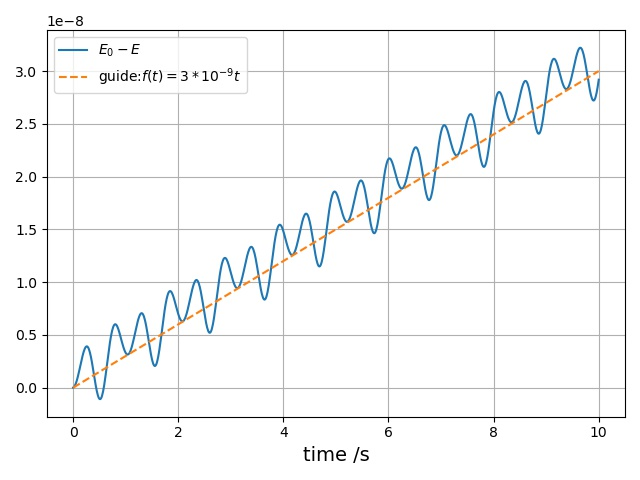
\includegraphics[scale=0.6]{figure/RK41/evaluation2/2021-2-9-223945.jpeg}
    \caption{系のエネルギー誤差の時間変化}
    \label{fig:RK41_eval2}
  \end{center}
\end{figure}
\newpage
\subsubsection{時間幅の取り方による誤差の変化}
今回用いているRunge-Kutta法は4次の精度を持つということが知られており,繰り返しの時間幅\(\Delta t\)を\(\dfrac{1}{10}\)倍すれば誤差は\(\dfrac{1}{10000}\)倍になるはずである.\\
したがって,この節では時間幅の取り方によって誤差がどのように変化しているかを確認する.\par
以下に示す図\ref{fig:RK41_eval1_1}から図\ref{fig:RK41_eval1_4}はソースコード\ref{src:RK41eval1}において,初角度をそれぞれ\(\dfrac{\pi}{2}\), \(\dfrac{\pi}{3}\), \(\dfrac{\pi}{4}\), \(\dfrac{\pi}{6}\)と設定して得られたグラフである.なお,ここでの誤差(Error)は10秒経過後の\(|E-E_0|\)と定義した.
\begin{figure}[H]
  \begin{center}
    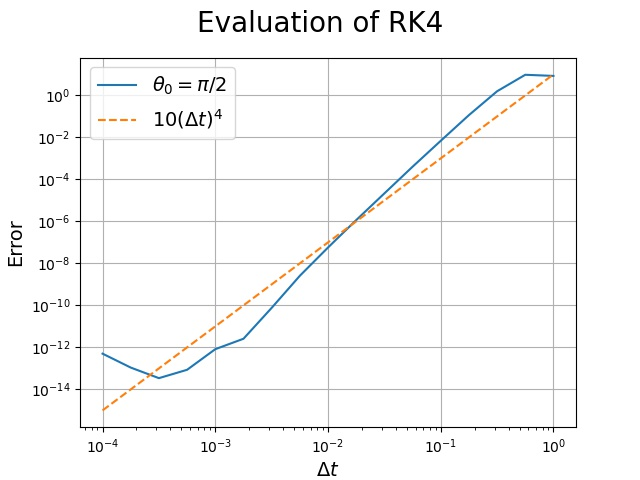
\includegraphics[scale=0.8]{figure/RK41/evaluation1/pi2_2021-2-9-222927.jpeg}
    \caption{初角度\(\dfrac{\pi}{2}における力学的エネルギーの精度\)}
    \label{fig:RK41_eval1_1}
  \end{center}
\end{figure}
\begin{figure}[H]
  \begin{center}
    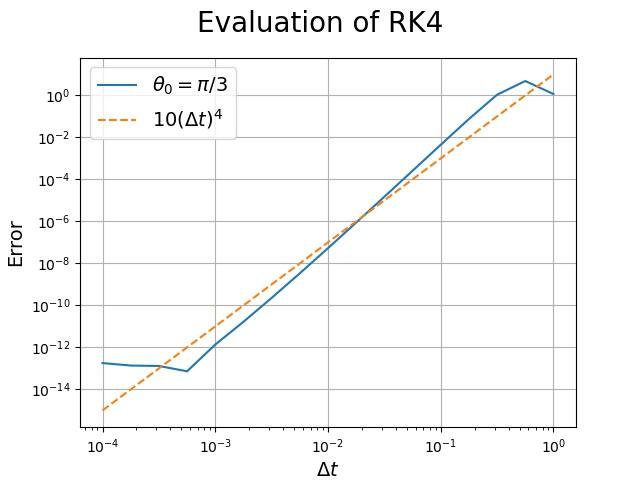
\includegraphics[scale=0.8]{figure/RK41/evaluation1/pi3_2021-2-9-222927.jpeg}
    \caption{初角度\(\dfrac{\pi}{3}における力学的エネルギーの精度\)}
    \label{fig:RK41_eval1_2}
  \end{center}
\end{figure}
\begin{figure}[H]
  \begin{center}
    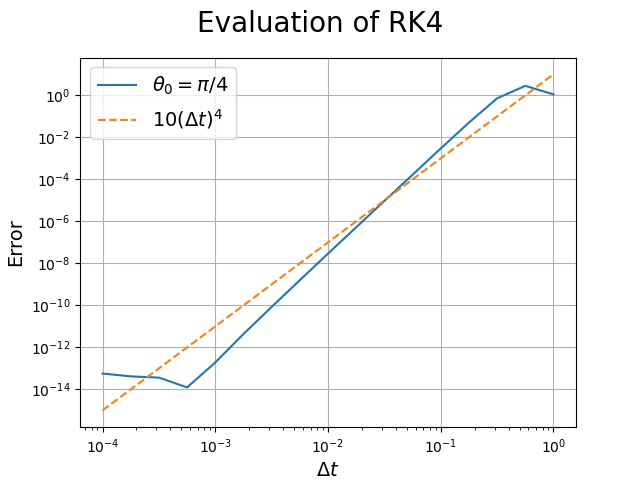
\includegraphics[scale=0.8]{figure/RK41/evaluation1/pi4_2021-2-9-222927.jpeg}
    \caption{初角度\(\dfrac{\pi}{4}における力学的エネルギーの精度\)}
    \label{fig:RK41_eval1_3}
  \end{center}
\end{figure}
\begin{figure}[H]
  \begin{center}
    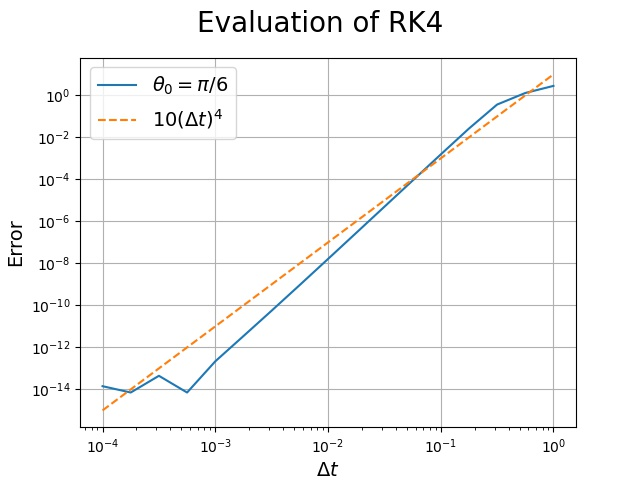
\includegraphics[scale=0.8]{figure/RK41/evaluation1/pi6_2021-2-9-222927.jpeg}
    \caption{初角度\(\dfrac{\pi}{6}における力学的エネルギーの精度\)}
    \label{fig:RK41_eval1_4}
  \end{center}
\end{figure}
\newpage
\subsection{考察}
まずアニメーションから読みとることのできる視覚的な情報についてであるが,ここからは運動のシミュレーションに不自然な点が特にないという事しか読み取ることができない.一方で振動の減衰などがはっきりと確認できるわけではないことから,系の力学的エネルギーがあまり変化していないのではないかという予想が立てられる.\par
次に,エネルギー誤差の時間変化についてである.\\
この図にひかれている点線は\(f(t) = 3\times10^{-9}t\)の補助線である.誤差は大域的にはこの直線に沿って増加し,局所的には振動している.ここに掲載した図\ref{fig:RK41_eval2}については初角度を\(\theta_0 = \dfrac{\pi}{4}\)としたものであるが,他の初角度に対しても同じような傾向(大域的には誤差が増加,局所的には振動)が確認できた.
振動しているように見える箇所は周期的に同じ形の変動を繰り返しているように見える.これは,それぞれの\(\theta\)について計算におけるエネルギーの減少しやすさや増加しやすさがある程度決まっており,そこを「周期的」に通るため同じような振動を繰り返しているように見えるのではないかと考えた.またそのように考えた場合,大域的に減少しているのは,「1周期」分の合計をとった時にその和が負の値であることによると考えられる(厳密な意味での周期的な運動ではないと考えられるため,「周期的」とあらわした).\par
最後に時間幅の変化に対する誤差の変化についてである.図\ref{fig:RK41_eval1_1}から図\ref{fig:RK41_eval1_4}の図中に記された点線は\(f(t) = 10(\Delta t)^{4}\)の補助線であり,4次の精度が達成されているかの目安となる.これらのグラフは両対数グラフになっていることに注意すると,この補助線よりも傾きが大きければ4次の精度を持っていると考えてよいと言える.\\
図より,どの初角度に対しても\(\Delta t = 10^0\)から\(\Delta t = 10^{-3}\)あたりにかけては4次の精度が成り立っている.一方で,\(\Delta t\)が\(10^{-3}\)よりも小さくなると誤差が増加傾向に転じる.これについて明確な理由はわかっていないが,上で述べたように,\(\theta\)に対応して誤差の変化のしやすさが決まっていると仮定し,\(\theta\)が大きい点(つまり角速度\(\omega\)が小さい点)における計算で誤差が広がりやすい場合を考えると,時間幅\(\Delta t\)が小さくなるにつれて\(\theta\)が大きい点で計算が実行される回数が増えていき,結果として一周期分の誤差増大量が大きくなると考えることができ辻褄が合う.\\
この仮定があっているかは,「1周期」分の計算においてどのような\(\theta\)で誤差が大きくなっているのかを確認すれば確かめられると考えたが,今回は時間不足で実施できなかった.

\newpage
\section{二重振り子の運動}
\subsection{二重振り子の運動方程式}

\subsection{二重振り子の運動方程式に対するRunge-Kutta法の適用}
\subsubsection{Runge-Kutta法の式について}
\subsubsection{Runge-Kutta法の妥当性について}
二重振り子の運動は\(\theta_1\),\ \(\theta_2\)が十分に小さいときのみ,近似を用いて解析解を求めることができる.したがって,微小角における解析解と数値解を比較することで,前節で定めたRunge-Kutta法の式による計算が妥当であるのかを確認することができる.\\
ここでは,\(\theta_1\),\ \(\theta_2 << 1\)である状況として,\(\theta_1 = \theta_2 = 0.001\),\ \(\dot{\theta_1} = \dot{\theta_2} = 0\)と設定する.

\subsection{結果}
\subsubsection{二重振り子の運動のアニメーション}

\subsubsection{エネルギー誤差の時間変化}

\subsubsection{時間幅の取り方による誤差の変化}

\newpage
\subsection{考察}

\newpage
\section{付録}
\subsection{二重振り子の運動方程式の導出}

\newpage
\subsection{二重振り子の微小角近似における解析解の導出}

\newpage
\subsection{ソースコード}
\lstinputlisting[caption=単振り子のアニメーション作成, label=src:RK41anim]{RK41_animation.py}
\newpage
\lstinputlisting[caption=単振り子におけるRK4の次数について, label=src:RK41eval1]{RK41_evaluation1.py}
\newpage
\lstinputlisting[caption=単振り子のエネルギーの時間変化について, label=src:RK41eval2]{RK41_evaluation2.py}
\newpage
\subsection{計算機環境}
\subsection{参考文献}
\end{document}